\chapter{Inference using nonlinear models}
\label{sec_inf_nonlin_mods}
In this chapter we consider probabilistic graphical models of the form shown in figure \ref{fig_nlmod}. These models have exactly the same form as the models in chapter \ref{sec_inf_lin_mods}. The variables retain their meaning as before but we generalise the model by dropping the linearity assumption. Unfortunately, this generalisation, although allowing us to expand our investigation to a much more expressive class of models, makes closed form solutions to the inference problem intractable in general.   
\begin{figure}[H] 
\centering
\begin{tikzpicture}

  % Define nodes
  \node[obs] (ya) {$y_0$};
  \node[obs, right=of ya] (yb) {$y_1$};
  \node[obs, right=of yb] (yc) {$y_2$};
  \node[latent, above=of ya]  (xa) {$x_0$};
  \node[latent, above=of yb, right=of xa]  (xb) {$x_1$};
  \node[latent, above=of yc, right=of xb]  (xc) {$x_2$};
  \node[det, above=of xa] (da) {$u_0$};
  \node[det, above=of xb] (db) {$u_1$};
  
  % Connect the nodes
  \edge {da} {xb};
  \edge {db} {xc};
  \edge {xa} {ya};
  \edge {xb} {yb};
  \edge {xc} {yc};
  \edge {xa} {xb};
  \edge {xb} {xc};
  
\end{tikzpicture}
\caption{Graphical model used in this chapter.}
\label{fig_nlmod}
\end{figure}
We again assume that the transition and observation functions are time invariant. The state space model is now of the form 
\begin{equation}
\begin{aligned}
x_{t+1} &= f(x_t, u_t, w_{t+1}) \\
y_{t+1} &= g(x_{t+1}, v_{t+1}).
\end{aligned}
\label{eq_nlstatespace}
\end{equation}
As in chapter \ref{sec_inf_lin_mods}, we observe $y_t$ to infer the latent $x_t$. Note that we make no assumption about the functional form of the noise terms $w_t,v_t$. In practice it is customary to assume that they have zero mean but otherwise are not restricted. Additionally, to simplify notation we will omit the dependence on $u$ of $f$ and $g$ and their associated distributions. Since $u$ is a deterministic variable, by assumption, it is straightforward to incorporate it into later analysis. 

\section{Sequential Monte Carlo methods}
\label{sec_asir}
Many approximate inference techniques exist in literature, the most notable ones include Gaussian sum filters \cite{gsf1} and particle based methods. We shall focus only on sequential Monte Carlo methods, of which particle based methods are a subset, because it is simple to implement and generalises well (and easily) to more complex graphical models. 

Sequential Monte Carlo methods are a general class of Monte Carlo methods which sample sequentially from a growing target distribution $\pi_t(x_{0:t})$. By only requiring that $\gamma_t$ be known point-wise we have the framework of sequential Monte Carlo methods in 
\begin{equation}
\begin{aligned}
\pi_t(x_{0:t}) &= \frac{\gamma_t(x_{0:t})}{Z_t} \\
Z_t &= \int_{x_{0:t}} \gamma_t(x_{0:t}).
\end{aligned}
\label{eq_SMC1}
\end{equation} 
Note that $Z_t$ is some normalisation constant \cite{pftut}.
For example, in the context of filtering we have that $\gamma_t(x_{0:t}) = p(x_{0:t},y_{0:t})$ and $Z_t = p(y_{0:t})$ so that $\pi_t(x_{0:t}) = p(x_{0:t}|y_{0:t})$. 

It is possible to approximate the distribution $\pi_t(x_{0:t})$ by drawing $N$ samples $X_{0:t}^i \backsim \pi_t(x_{0:t})$ and using the Monte Carlo method to find the approximation $\hat{\pi}_t(x_{0:t})$ by
\begin{equation}
\pi_t(x_{0:t}) \approx \hat{\pi}_t(x_{0:t}) = \frac{1}{N}\sum_{i=1}^N \delta(X^i_{0:t}, x_{0:t}).
\label{eq_SMC2}
\end{equation}
We denote the Dirac delta function of $x$ with mass located at $x_0$ by $\delta(x_0,x)$. It is easy to approximate the marginal $\pi_t(x_{t})$ as
\begin{equation}
\hat{\pi}_t(x_{t}) = \frac{1}{N}\sum_{i=1}^N \delta(X^i_{t}, x_{t}).
\label{eq_SMC3}
\end{equation}
It can be shown that the variance of the approximation error of $\pi_t$ decreases at rate $\mathcal{O}(\frac{1}{N})$. Unfortunately there are two significant drawbacks to the Monte Carlo approximation. The first is that often we cannot sample from $\pi_t(x_{0:t})$ directly and the second is that even if we could it is often computationally prohibitive. 

We use the importance sampling method to address the first problem. We do this by introducing an importance (sometimes called proposal) density $q_t(x_{0:t})$ such that $\pi_t(x_{0:t}) > 0 \implies q_t(x_{0:t}) > 0$. By substituting this into the sequential Monte Carlo framework (\ref{eq_SMC1}) we have
\begin{equation}
\begin{aligned}
\pi_t(x_{0:t}) &= \frac{w_t(x_{0:t})q_t(x_{0:t})}{Z_t} \\
Z_t &= \int_{x_{0:t}} w_t(x_{0:t})q_t(x_{0:t}).
\end{aligned}
\label{eq_SMC4}
\end{equation} 
Where we have defined the unnormalised weight function $w_t(x_{0:t}) = \frac{\gamma_t(x_{0:t})}{q_t(x_{0:t})}$. It is possible, for example, to set $q_t$ to a multivariate Gaussian which is easy to sample from. By drawing $N$ samples $X_{0:t}^i \backsim q_t(x_{0:t})$ and using (\ref{eq_SMC4}) we have 
\begin{equation}
\begin{aligned}
\hat{\pi}_t(x_{0:t}) &= \frac{1}{N}\sum_{i=1}^N W_t^i\delta(X^i_{0:t}, x_{0:t}) \\
\hat{Z}_t &= \frac{1}{N}\sum_{i=1}^N w_t(X^i_{0:t}) \\
W^i_t &= \frac{w_t(X^i_{0:t})}{\sum_{i=1}^N w_t(X^i_{0:t})}.
\end{aligned}
\label{eq_SMC5}
\end{equation}
Now we will attempt to modify the importance sampling method to address the second problem of computational cost incurred by the sampling routine. 

We do this by selecting an importance/proposal distribution which factorises according to $q_t(x_{0:t}) = q_{t-1}(x_{0:t-1})q_t(x_{t}|x_{0:t-1}) = q_0(x_0) \Pi_{k=1}^t q_k(x_k|x_{0:k-1})$. In this way we only need to sample sequentially at each time step: at time $t=0$ we sample $X_0^i \backsim q_0(x_0)$, at time $t=1$ we sample $X_{1}^i \backsim q_1(x_1|x_0)$ and so we build up $X^i_{0:t} \backsim q_t(x_{0:t})$ factor by factor.

The weights can be written in the form
\begin{equation}
\begin{aligned}
w_t(x_{0:t}) &= \frac{\gamma_t(x_{0:t})}{q_t(x_{0:t})} \\
&= \frac{\gamma_{t-1}(x_{0:t-1})}{q_{t-1}(x_{0:t-1})}\frac{\gamma_t(x_{0:t})}{\gamma_{t-1}(x_{0:t-1})q_t(x_t|x_{0:t-1})} \\
&= w_{t-1}(x_{0:t-1})\alpha_t(x_{0:t-1}) \\
&= w_0(x_0)\Pi_{k=1}^t \alpha_k(x_{0:k}).
\end{aligned}
\label{eq_SMC6}
\end{equation}
Thus, at any time $t$ we can obtain the estimates $\hat{\pi}_t(x_{0:t})$ and $Z_t$. The major limitation of this approach is that the variance of the resulting estimates typically increases exponentially with $t$ \cite{pftut}. 

We overcome this problem by resampling and thus introduce the sequential importance resampling method. So far we have a set of weighted samples generated from $q_t(x_{0:t})$ which builds the approximation $\hat{\pi}_t(x_{0:t})$. However, sampling directly from $\hat{\pi}_t(x_{0:t})$ does not approximate $\pi_t(x_{0:t})$. To obtain an approximate distribution of $\pi_t(x_{0:t})$ we need to sample from the weighted distribution $\hat{\pi}_t(x_{0:t})$. This is called resampling because we are sampling from a sampled distribution. Many techniques exist to perform this step efficiently. The crudest and most widely used one is to simply use the discrete multinomial distribution based on $W^i_{0:t}$ to draw samples from $\hat{\pi}_t(x_{0:t})$ \cite{pftut}. 

The benefit of resampling is that it allows us to remove particles with low weight and thus keeps the variance of the estimate in check. We are finally ready to consider the general sequential importance resampling algorithm:

\textbf{Sequential importance resampling algorithm} \\
For $t=0$:
\begin{enumerate}
\item
Sample $X^i_0 \backsim q_0(x_0)$.
\item
Compute the weights $w_0(X_0^i)$ and $W^i_0 \propto w_0(X^i_0)$.
\item
Resample $(W^i_0, X^i_0)$ to obtain $N$ equally weighted particles $(\frac{1}{N}, \bar{X}^i_0)$.
\end{enumerate}
For $t \geq 1$:
\begin{enumerate}
\item
Sample $X^i_t \backsim q_t(x_t|\bar{X}^i_{0:t-1})$ and set ${X}^i_{0:t} \leftarrow (\bar{X}^i_{0:t-1}, X^i_t)$ .
\item
Compute the weights $\alpha_t(X^i_{0:t})$ and $W^i_t \propto \alpha_t(X^i_{0:t})$.
\item
Resample $(W^i_t, X^i_{0:t})$ to obtain $N$ equally weighted particles $(\frac{1}{N}, \bar{X}^i_{0:t})$.
\end{enumerate}
At any time $t$ we have two approximations for $\pi(x_{0:t})$:
\begin{equation}
\begin{aligned}
\hat{\pi}(x_{0:t}) &= \sum_{i=1}^N W^i_t \delta(X^i_{0:t}, x_{0:t}) \\
\bar{\pi}(x_{0:t}) &= \frac{1}{N}\sum_{i=1}^N \delta(\bar{X}^i_{0:t}, x_{0:t}).
\end{aligned}
\label{eq_smc_algo}
\end{equation}
The latter approximation represents the resampled estimate and the former represents the sampled estimate \cite{pftut}. We prefer the former because in the limit as $N \rightarrow \infty$ it is a better approximation of $\pi_t$. However, as we have mentioned the variance of $\hat{\pi}(x_{0:t})$ tends to be unbounded and thus we often have that most of the particles in the particle population have very low weight. From a computational point of view this is wasteful. To ameliorate this we use the latter, resampled, estimate. However, the problem with the resampled estimate is that it effectively culls low weight particles and this reduces the diversity of the particle population \cite{murphy1}. 

We attempt to get the benefit of both worlds by only performing resampling when the weight variance of the particles becomes large. The effective sample size (ESS) is a method whereby one determines when to perform resampling according to 
\begin{equation}
\text{ESS} = \frac{1}{\sum_{i=1}^N (W^i_n)^2}.
\label{eq_ess}
\end{equation} 
If the effective sample size becomes smaller than some threshold (typically $\frac{N}{2}$) we resample to cull low weight particles and replace them with high weight particles. In this manner we have a computationally feasible method. This is called adaptive resampling and is a straightforward extension of the sequential Monte Carlo algorithm as shown below.

\textbf{Adaptive sequential importance resampling algorithm}\\
For $t=0$:
\begin{enumerate}
\item
Sample $X^i_0 \backsim q_0(x_0)$.
\item
Compute the weights $w_0(X_0^i)$ and $W^i_0 \propto w_0(X^i_0)$.
\item
If resample criterion is satisfied then resample $(W^i_0, X^i_0)$ to obtain $N$ equally weighted particles $(\frac{1}{N}, \bar{X}^i_0)$ and set $(\bar{W}^i_0, \bar{X}^i_0) \leftarrow (\frac{1}{N}, \bar{X}^i_0)$ otherwise set $(\bar{W}^i_0, \bar{X}^i_0) \leftarrow ({W}^i_0, {X}^i_0)$.
\end{enumerate}
For $t \geq 1$:
\begin{enumerate}
\item
Sample $X^i_t \backsim q_t(x_t|\bar{X}^i_{0:t-1})$ and set ${X}^i_{0:t} \leftarrow (\bar{X}^i_{0:t-1}, X^i_t)$ .
\item
Compute the weights $\alpha_t(X^i_{0:t})$ and $W^i_t \propto \bar{W}^i_{t-1}\alpha_t(X^i_{0:t})$.
\item
If the resample criterion is satisfied then resample $(W^i_t, X^i_{0:t})$ to obtain $N$ equally weighted particles $(\frac{1}{N}, \bar{X}^i_{0:t})$ and set $(\bar{W}^i_1, \bar{X}^i_t) \leftarrow (\frac{1}{N}, \bar{X}^i_t)$ otherwise set $(\bar{W}^i_t, \bar{X}^i_t) \leftarrow ({W}^i_t, {X}^i_t)$.
\end{enumerate}

Numerous convergence results exist for the sequential Monte Carlo methods we have discussed but the fundamental problem with this scheme is that of sample impoverishment. It is fundamentally impossibly to accurately represent a distribution on a space of arbitrarily high dimension with a finite set of samples \cite{pftut}. We attempt to mitigate this problem by using resampling but degeneracy inevitably occurs for large enough $t$. Fortunately, for our purposes we will not be dealing with arbitrarily large dimensional problems because of the Markov assumption.

\section{Particle filter}
\label{sec_bootstrap}
We now apply the adaptive sequential importance resampling algorithm in the setting of filtering. We set $\pi_t(x_{0:t}) = p(x_{0:t}|y_{0:t})$, $\gamma_t(x_{0:t}) = p(x_{0:t}, y_{0:t})$ and consequently $Z_t = p(y_{0:t})$. We use the recursive proposal distribution $q_t(x_{0:t}|y_{0:t}) = q(x_t|x_{0:t-1}, y_{0:t})q_{t-1}(x_{0:t-1}|y_{0:t-1})$. We then have the unnormalised weights
\begin{equation}
\begin{aligned}
w_t(x_{0:t}) &= \frac{\gamma_t(x_{0:t})}{q_t(x_{0:t}|y_{0:t})} \\
&= \frac{p(x_{0:t}, y_{0:t})}{q_t(x_{0:t}|y_{0:t})} \\
&\propto \frac{p(x_{0:t}| y_{0:t})}{q_t(x_{0:t}|y_{0:t})} \\
&\propto \frac{p(y_t|x_t)p(x_t|x_{t-1})}{q_t(x_t|x_{0:t-1}, y_{0:t})}\frac{p(x_{0:t-1}| y_{0:t-1})}{q_{t-1}(x_{0:t-1}|y_{0:t-1})} \\
&= \alpha_t(x_{0:t})w_{t-1}(x_{0:t-1}).
\end{aligned}
\label{eq_pf_weights}
\end{equation}
For filtering we only care about $p(x_t|y_{0:t})$ and thus we do not need the entire trajectory $x_{0:t}$. This allows us to choose the proposal distribution $q_t(x_t|x_{0:t-1}, y_{0:t}) = q_t(x_{t}|x_{t-1}y_{t})$. In this case the incremental weight $\alpha_t$ simplifies to
\begin{equation}
\alpha_t(x_{0:t}) = \frac{p(y_t|x_t)p(x_t|x_{t-1})}{q_t(x_t|x_{t-1}, y_{t})}.
\label{eq_pf_simpweights}
\end{equation}
The most common proposal distribution is, the suboptimal, $q_t(x_t|x_{t-1}|y_t) = p(x_t|x_{t-1})$ because it is easy to sample from. This implies that the incremental weights simplify to $\alpha_t(x_{0:t}) = p(y_t|x_t)$. Using such a proposal distribution was initially proposed in \cite{gordon} in the setting of the non-adaptive sequential importance resampling method. 

For general purpose filtering this is not very efficient because it amounts to ``guessing until you hit". If the transitions are very stochastic inference can be improved by using the optimal proposal distribution $q_t(x_t|x_{t-1}, y_t) = p(x_t|x_{t-1}, y_t)$. While this is optimal it introduces some difficulty because, in general, it is more difficult to sample from. The focus of dissertation is not on optimal filtering and for the purposes of prediction the suggested proposal distribution is sufficiently good \cite{murphy1}. We thus restrict ourselves to the proposal distribution $p(x_t|x_{t-1})$ for simplicity.

Finally, we have mentioned that resampling kills off unlikely particles. An unfortunate consequence of this is that some particle diversity is lost. An empirical method used to attenuate this problem is to resample from a kernel around the particle selected by the resampling process. This is called roughening in \cite{gordon}. We thus make a final modification to the adaptive sequential importance resampling algorithm. We select a particle from the population in the standard way but resample from a normal distribution centred around that particle and with a diagonal covariance matrix where the standard deviation of each diagonal is $KEN^{-\frac{1}{d}}$. We define $E$ as the range of the particle's relevant component, $N$ as the number of particles and $d$ as the dimension of the problem. $K$ is a tuning factor which specifies how broad the kernel we sample from should be. 

For the sake of completeness we present the particle filter algorithm we used here. Recall that $f$ and $g$ are the transition and observation functions respectively. The algorithm is applied to each particle $i=1,2,...,N$.

\textbf{Particle filter algorithm}\\
For $t=0$:
\begin{enumerate}
\item
Sample $X^i_0 \backsim p(x_0)$.
\item
Compute the weights $w_0(X_0^i) = p(y_0|X_0^i) = \mathcal{N}(y_0|g(X^i_0), V)$ where $y_0$ is the observation. Normalise $W^i_0 \propto w_0(X^i_0)$.
\item
If the number of effective particles is below some threshold apply resampling with roughening $(W^i_0, X^i_0)$ to obtain $N$ equally weighted particles $(\frac{1}{N}, \bar{X}^i_0)$ and set $(\bar{W}^i_0, \bar{X}^i_0) \leftarrow (\frac{1}{N}, \bar{X}^i_0)$ otherwise set $(\bar{W}^i_0, \bar{X}^i_0) \leftarrow ({W}^i_0, {X}^i_0)$
\end{enumerate}
For $t \geq 1$:
\begin{enumerate}
\item
Sample $X^i_t = f(\bar{X}^i_{t-1}, w_t) \backsim p(x_t|\bar{X}^i_{t-1}, W)$.
\item
Compute the weights $\alpha_t(X^i_{t}) = p(y_t|X_t^i) = \mathcal{N}(y_t|g(X^i_t), V)$ and normalise $W^i_t \propto \bar{W}^i_{t-1}\alpha_t(X^i_{t})$.
\item
If the number of effective particles is below some threshold apply resampling with roughening $(W^i_t, X^i_{t})$ to obtain $N$ equally weighted particles $(\frac{1}{N}, \bar{X}^i_{t})$ and set $(\bar{W}^i_1, \bar{X}^i_t) \leftarrow (\frac{1}{N}, \bar{X}^i_t)$ otherwise set $(\bar{W}^i_t, \bar{X}^i_t) \leftarrow ({W}^i_t, {X}^i_t)$.
\end{enumerate}
The algorithm presented above is a slight generalisation of the bootstrap particle filter as initially proposed by Gordon et. al. \cite{gordon}.

Intuitively the algorithm may be summarised like this: particle filters predict the next hidden state by projecting all the current particles forward using the transition function and associated noise. For each particle the likelihood of the observation is calculated given the particle and measurement noise. This likelihood is related to the weight of each particle. Particles with a relatively high weight are then deemed to more accurately represent the posterior distribution and thus we infer the posterior state estimate based on the relative weights of each particle. The graphical model of particle filtering is exactly the same as that of the Kalman filter graphical model as shown in figure \ref{fig_gm_linmods_filtering}. This should not come as a surprise because the general graphical model of this chapter, figure \ref{fig_nlmod}, is exactly the same as the general graphical model of chapter \ref{sec_inf_lin_mods} as shown in figure \ref{fig_linmod2}. 

\section{Particle prediction}
\label{sec_particle_prediction}
We are primarily interested in predicting the future hidden states but we also show how the future visible states may be predicted within the framework of particle based methods. Recalling the prediction derivations of chapter \ref{sec_hmm} and chapter \ref{sec_inf_lin_mods} we expect the hidden state prediction to merely be an $n$ step ahead projection of the current filtered particles. Likewise, we expect the visible state prediction to just be transformation of the predicted hidden states under the observation function. 

Inspecting the bootstrap particle filter algorithm presented in section \ref{sec_bootstrap} we are relieved to find that this is the case. One just removes the observation update steps (steps 2 and 3) from the algorithm because we cannot observe the future. We illustrate the two step ahead predictions and trust that the reader can generalise from here.

\textbf{Particle Prediction Algorithm}
\begin{enumerate}
\item
Sample $X_{t+1}^i = f(\bar{X}_t^i, w_{t+1}) \backsim p(x_{t+1}^i|y_t, \bar{X}_t^i)$ 
\item
Project $X_{t+2}^i = f(X_{t+1}^i, w_{t+2}) \backsim p(x_{t+2}^i|y_t, X_{t:t+1}^i)$ 
\item
Project $Y_{t+2}^i = g(X_{t+2}^i, v_{t+2}) \backsim p(y_{t+2}^i|y_t, X_{t:t+1}^i)$ 
\end{enumerate}
Once again, the graphical model depicting this situation is exactly the same as figure \ref{fig_gm_linmods_prediction} for the same reasons as mentioned before.

\section{Smoothing and Viterbi decoding}
In the context of nonlinear transition and observation functions smoothing and Viterbi decoding are much more difficult than before. For the purposes of this dissertation it is not important to consider inferences of that type and thus we merely refer the reader to literature where this is discussed \cite{barber}\cite{pftut}\cite{gsf1}\cite{murphy1}\cite{murphy2}.

\section{Filtering the CSTR}
\label{sec_nonlinmods_filtering}
In this chapter we apply the particle filter to the nonlinear CSTR problem introduce in chapter \ref{sec_cstr}. We first demonstrate the effectiveness of the particle filter by performing inference using the full nonlinear CSTR model measuring only temperature. Next we use the full nonlinear model again but measure both temperature and concentration. Finally, we compare the particle filter and the Kalman filter measuring both states. These investigations are by no means thorough but serve to illustrate important aspects of probabilistic graphical models which will affect control.

We do not investigate the effect the number of particles used for inference has on the particle filter. It is well known that increasing the number of particles increases the accuracy of particle based methods \cite{murphy1} but at the cost of increased computational complexity. The number of particles used in this dissertation reflects this trade-off i.e. we use a relatively small number of particles so that the simulations run quickly but are still accurate enough for practical purposes. 

Although it is not necessary we assume that the process and measurement noise is Gaussian with the same distributions as those found in section \ref{sec_filtering_linmods}. This holds for all the other parameters as well. We have used 200 particles to represent the state posterior. In figure \ref{fig_pf_m1_time} we see the state estimates as a function of time.
\begin{figure}[H] 
\centering
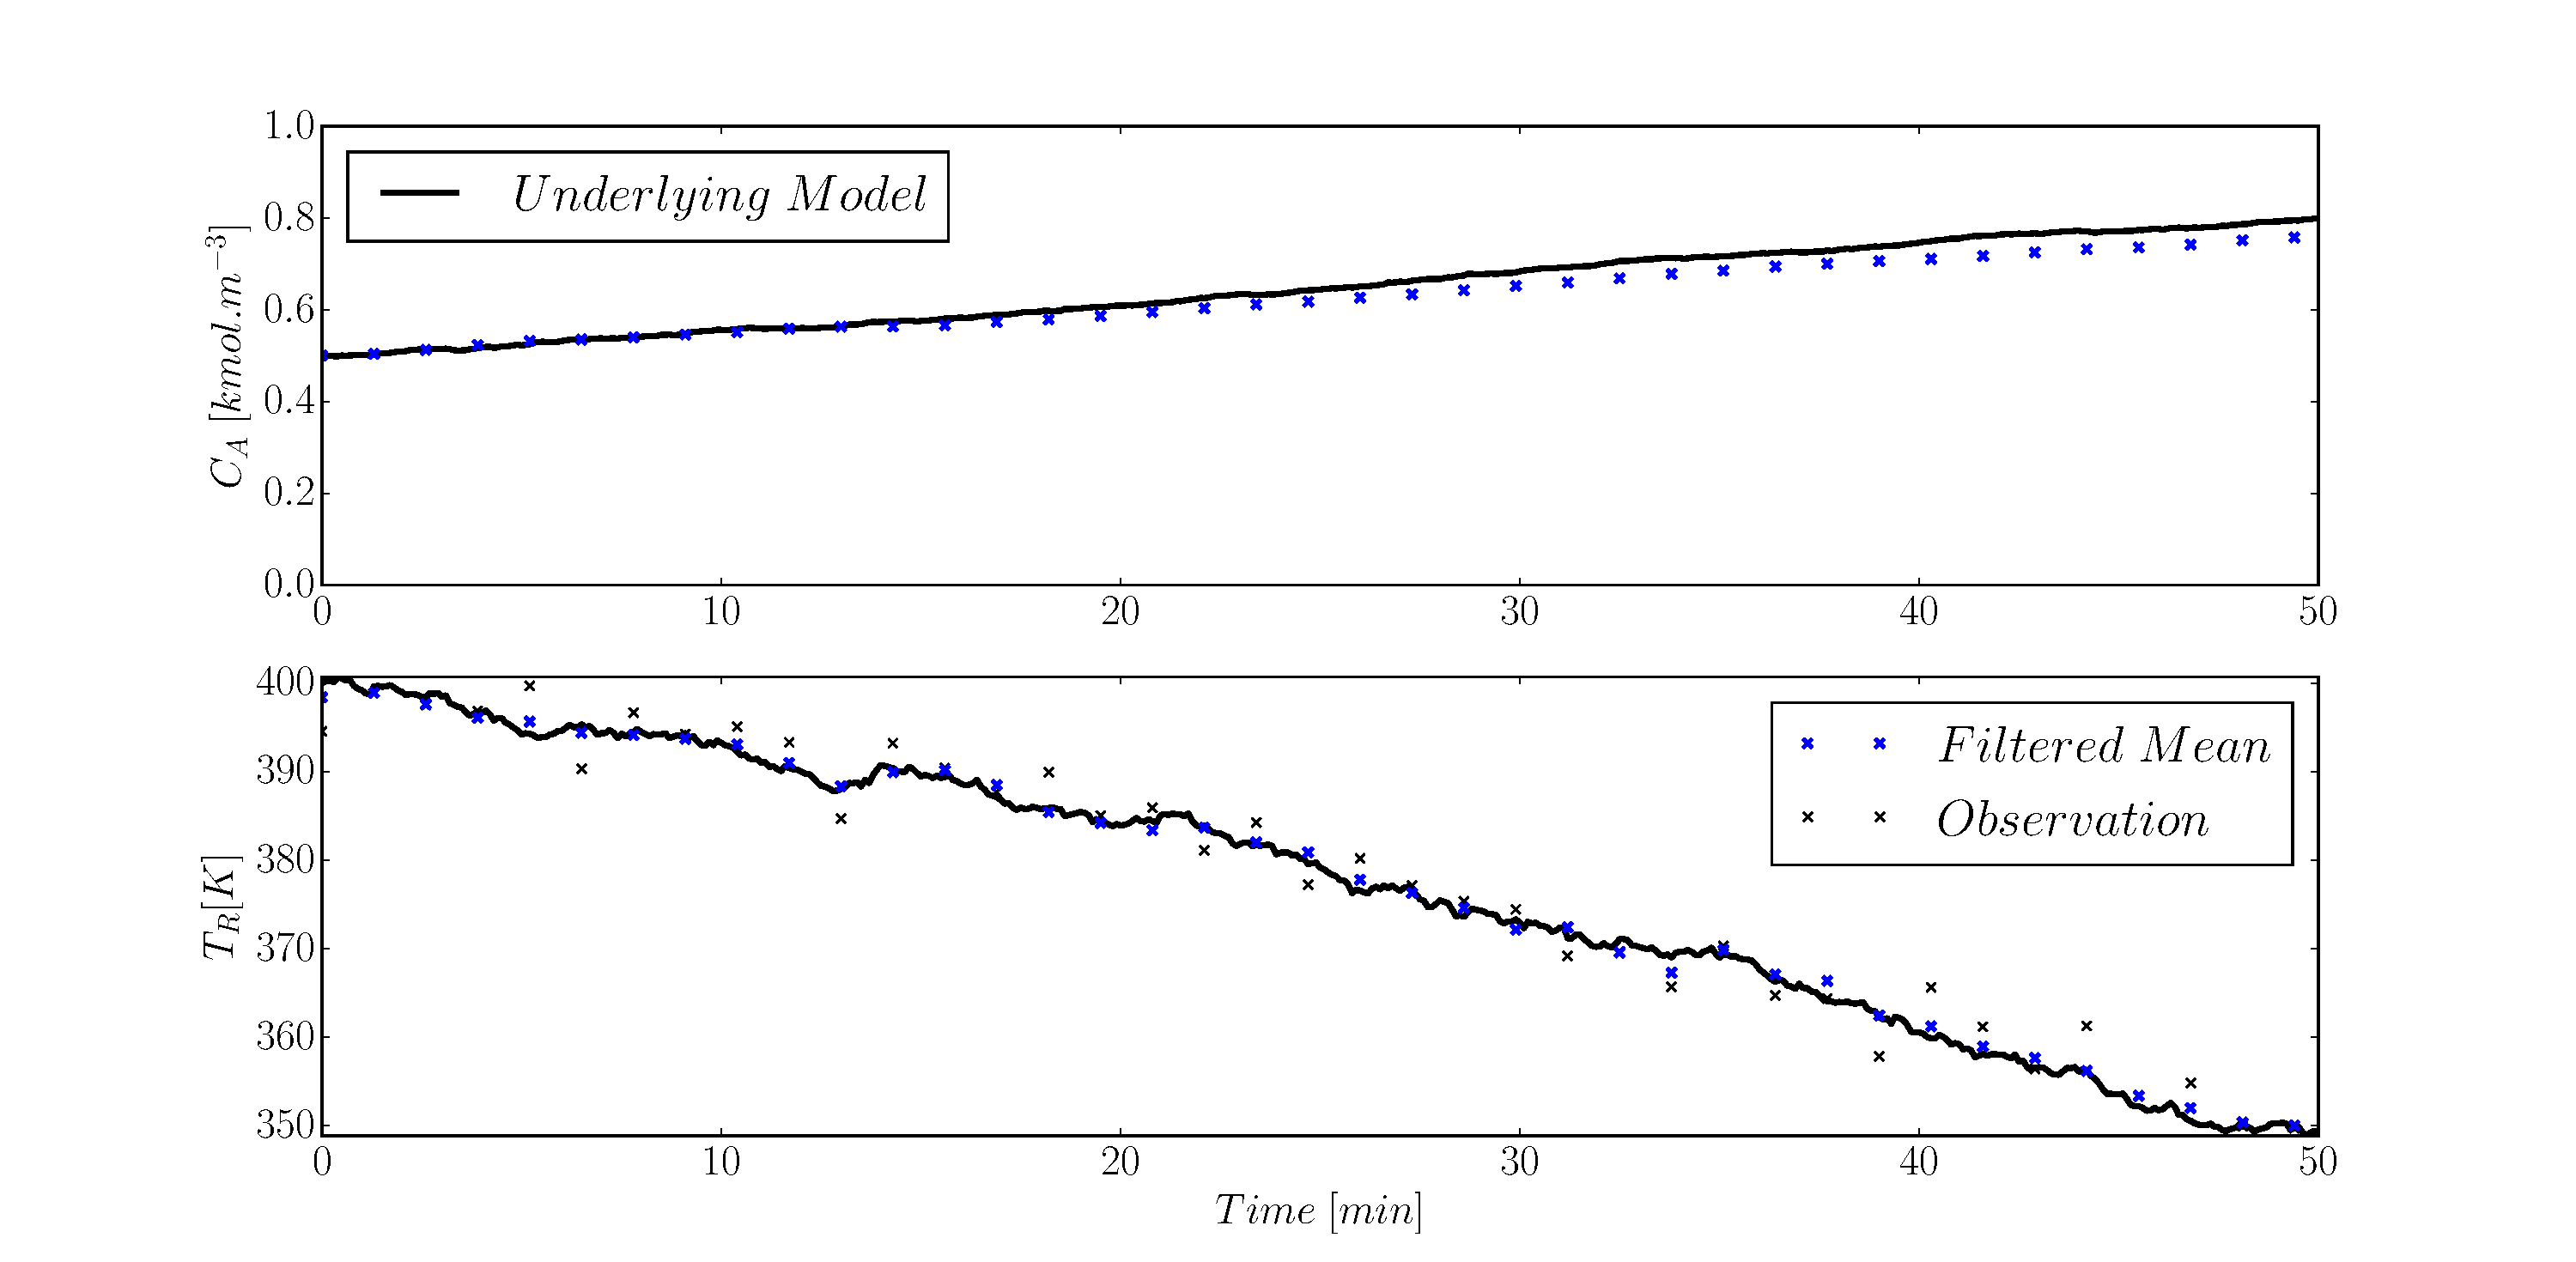
\includegraphics[width=\textwidth]{pf_m1_time.pdf}
\caption{Time series state estimates using the particle filter on the nonlinear CSTR model with initial condition $(0.5, 400)$ and measuring only temperature. The filter uses 200 particles.}
\label{fig_pf_m1_time}
\end{figure}
The filter tracks both states reasonable well with a little more variance evident in the unmeasured state. The benefit of using the full nonlinear model is evident here - since the model is more accurate than the previously used linear model the filter infers the concentration more accurately. The average concentration and temperature estimation error is 3.15\% and 0.20\% respectively. Compare this to 22.73\% and 0.47\% over the same simulation time using a Kalman filter measuring only temperature. The increased accuracy is also reflected in the state space evolution curve in figure \ref{fig_pf_m1_phase}.
\begin{figure}[H] 
\centering
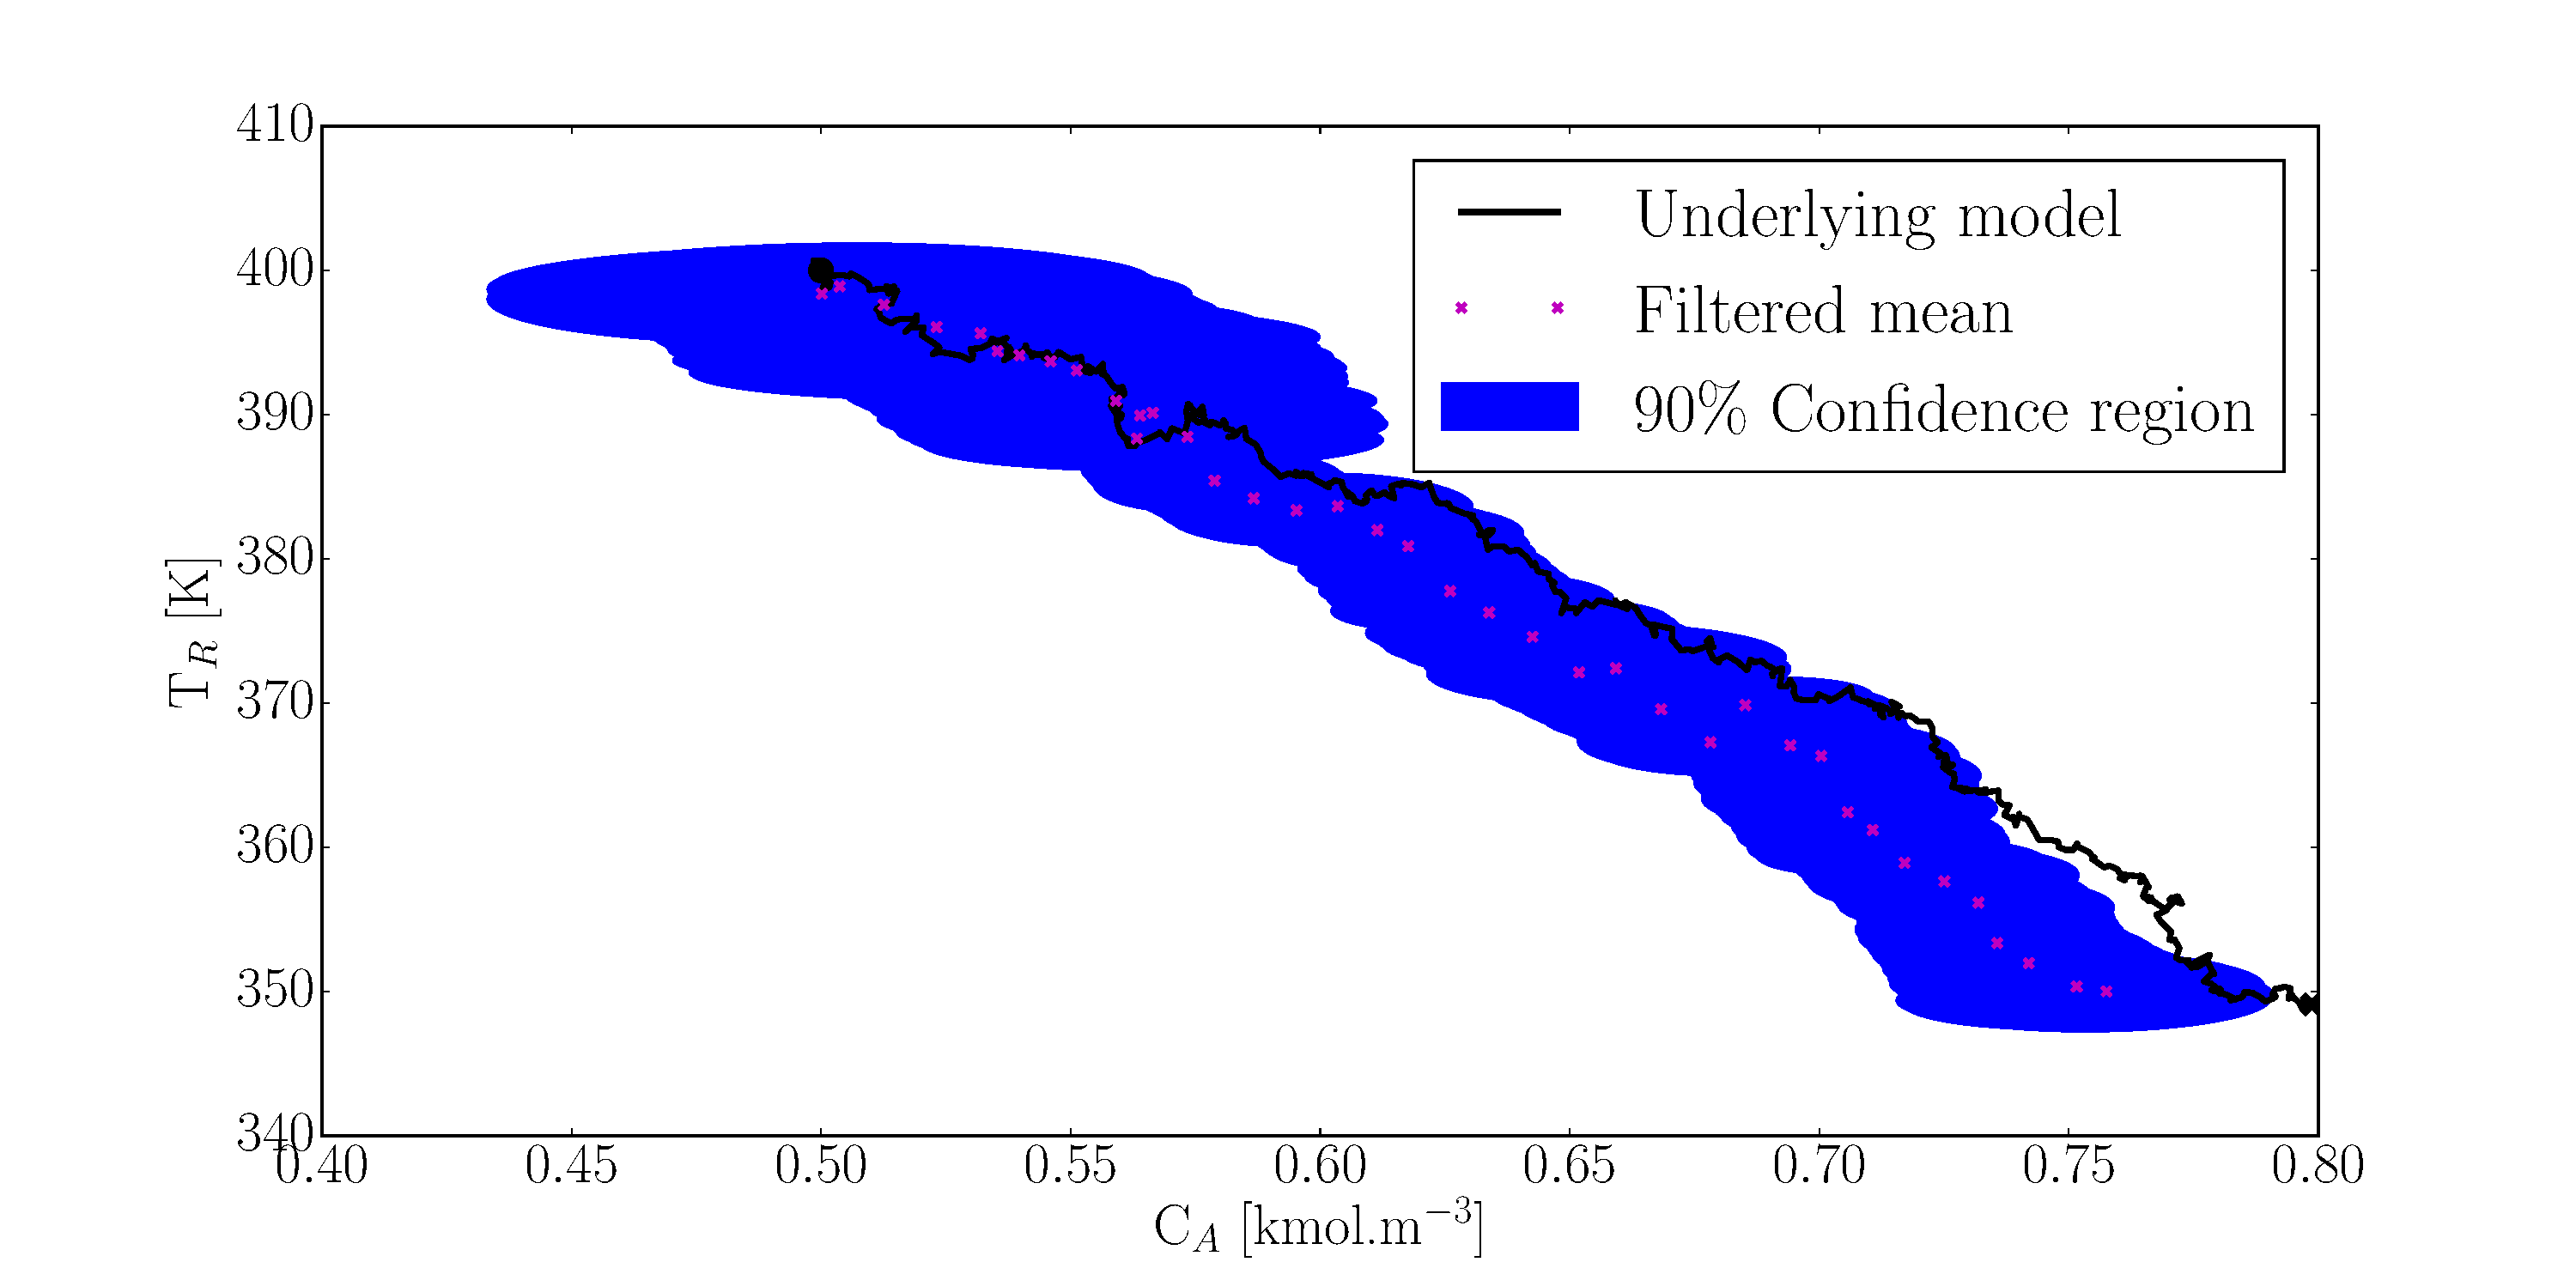
\includegraphics[width=\textwidth]{pf_m1_phase.pdf}
\caption{State space evolution of the particle filter on the nonlinear CSTR model with initial condition $(0.5, 450)$ and measuring only temperature. The filter uses 200 particles.}
\label{fig_pf_m1_phase}
\end{figure}
We also see in figure \ref{fig_pf_m1_phase} that the variance of the estimates is quite high (the confidence region is quite big). We expect that by also measuring concentration this will decrease. In figures \ref{fig_pf_m2_time} and \ref{fig_pf_m2_phase} we incorporate concentration measurement to aid inference. 
\begin{figure}[H] 
\centering
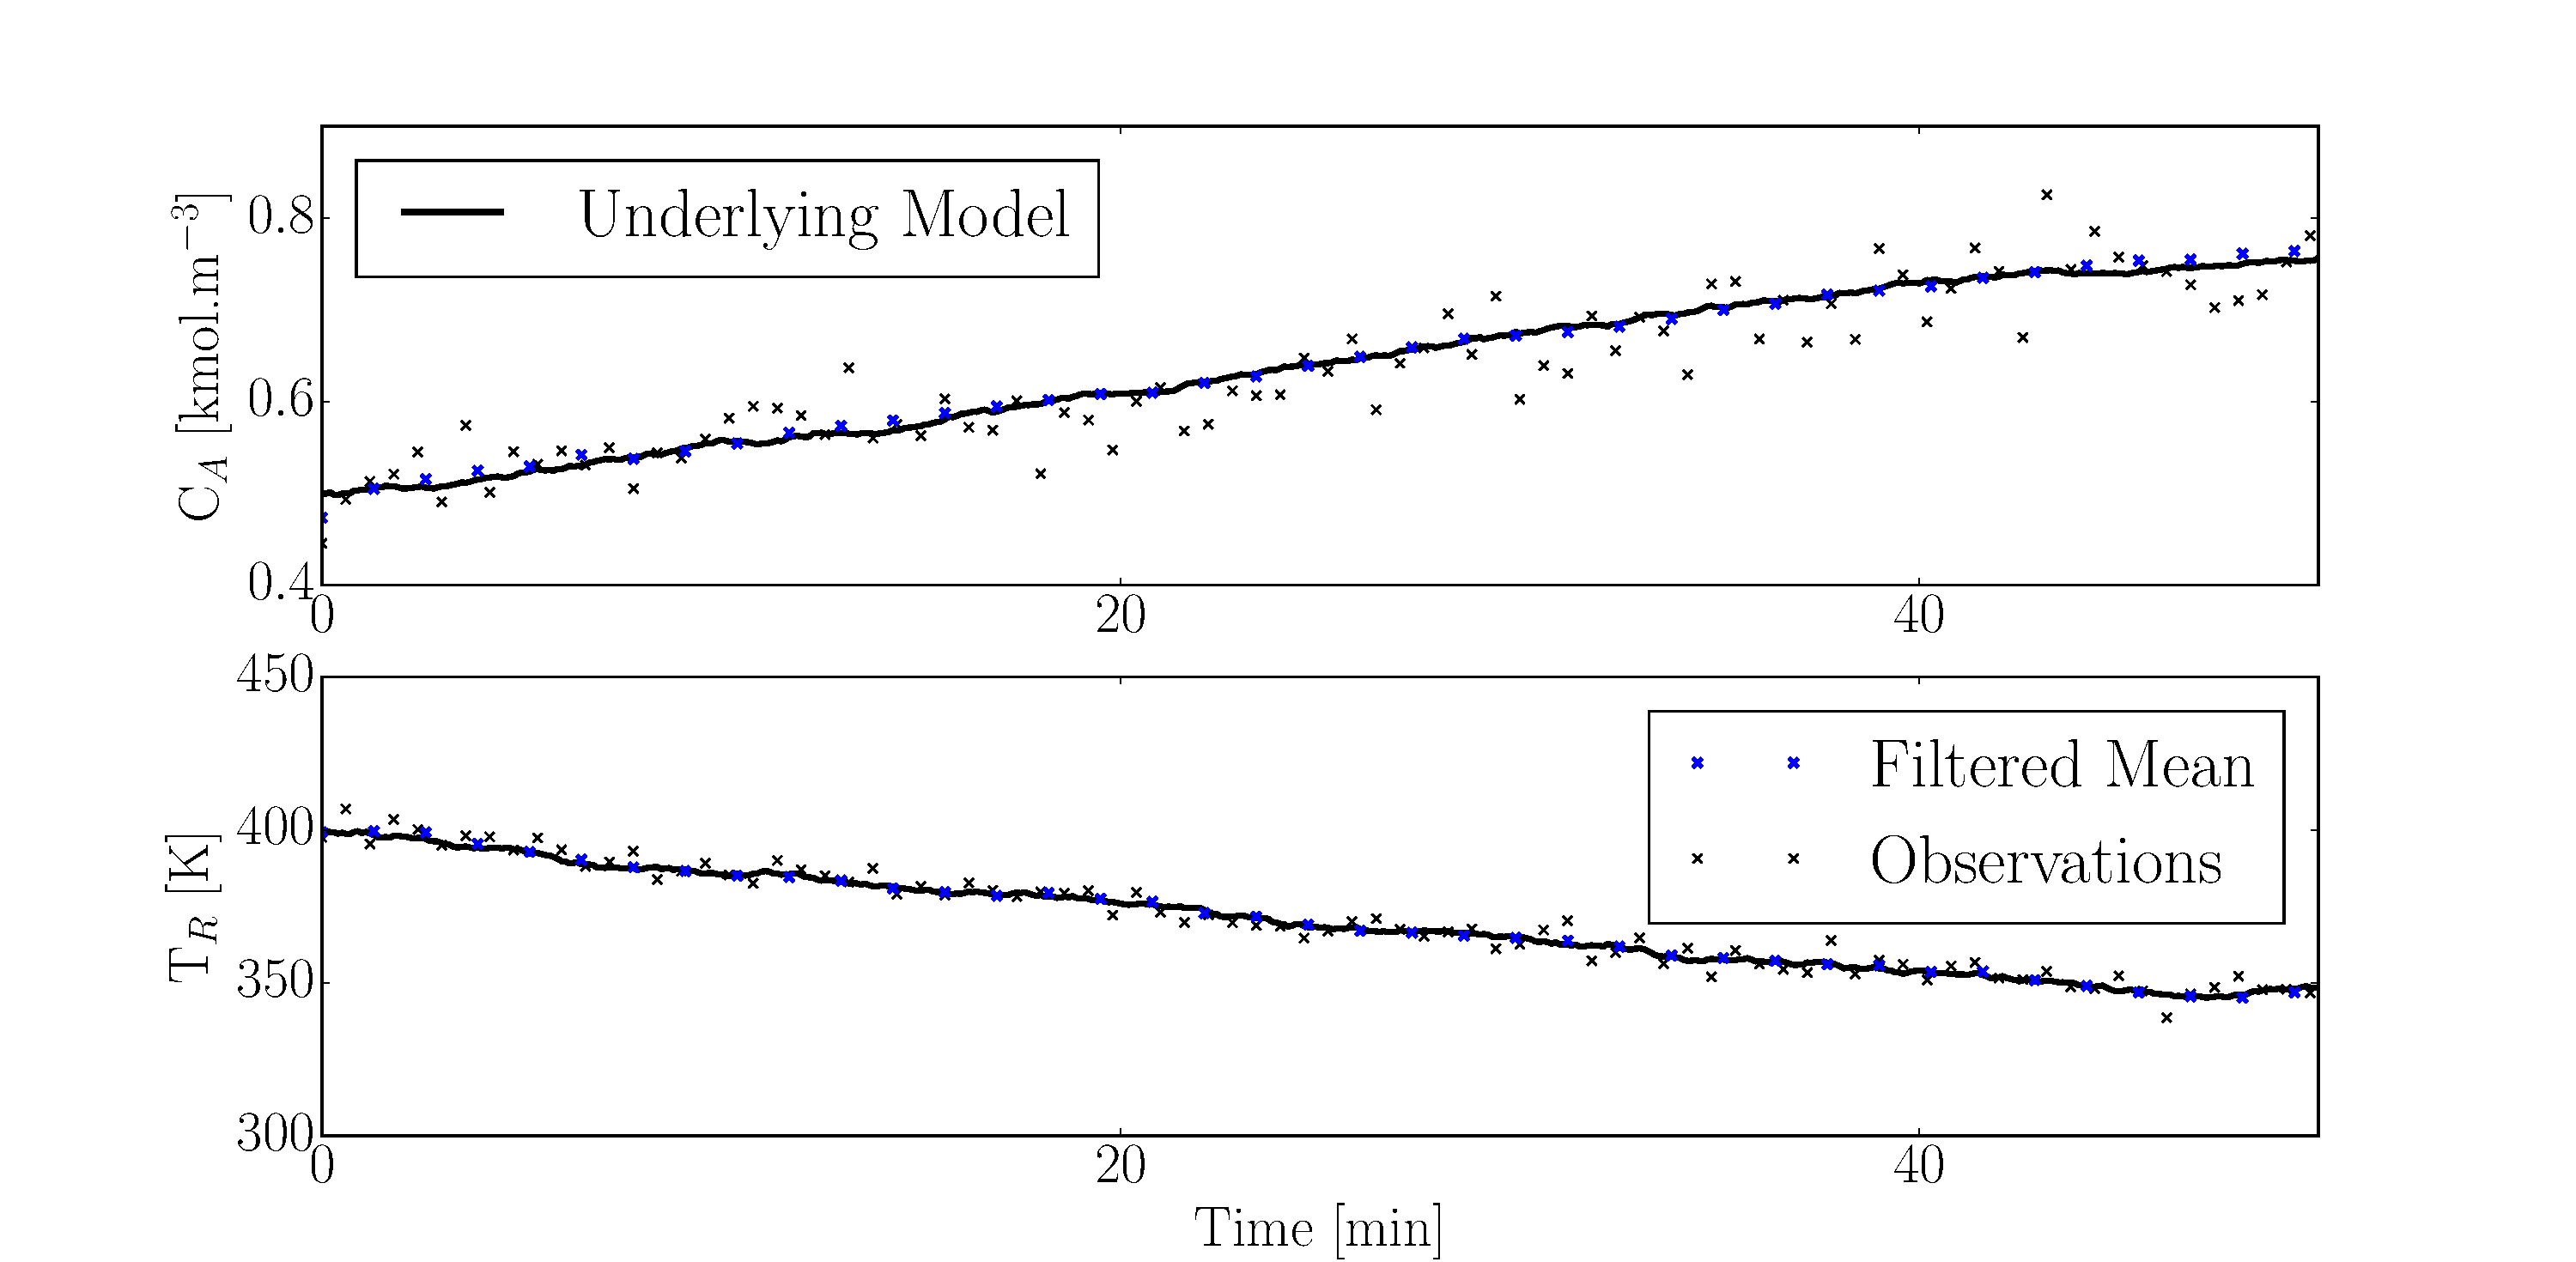
\includegraphics[width=\textwidth]{pf_m2_time.pdf}
\caption{Time series state estimates using the particle filter on the nonlinear CSTR model with initial condition $(0.5, 450)$ and measuring both states. The filter uses 200 particles.}
\label{fig_pf_m2_time}
\end{figure}
It is clear that that the particle filter reliably tracks the state evolution in the presence of plant and measurement noise. The average concentration and temperature estimation error is 0.81\% and 0.21\% respectively. We see that by also measuring the concentration the size of the confidence region decreases in figure \ref{fig_pf_m2_phase}. 
\begin{figure}[H] 
\centering
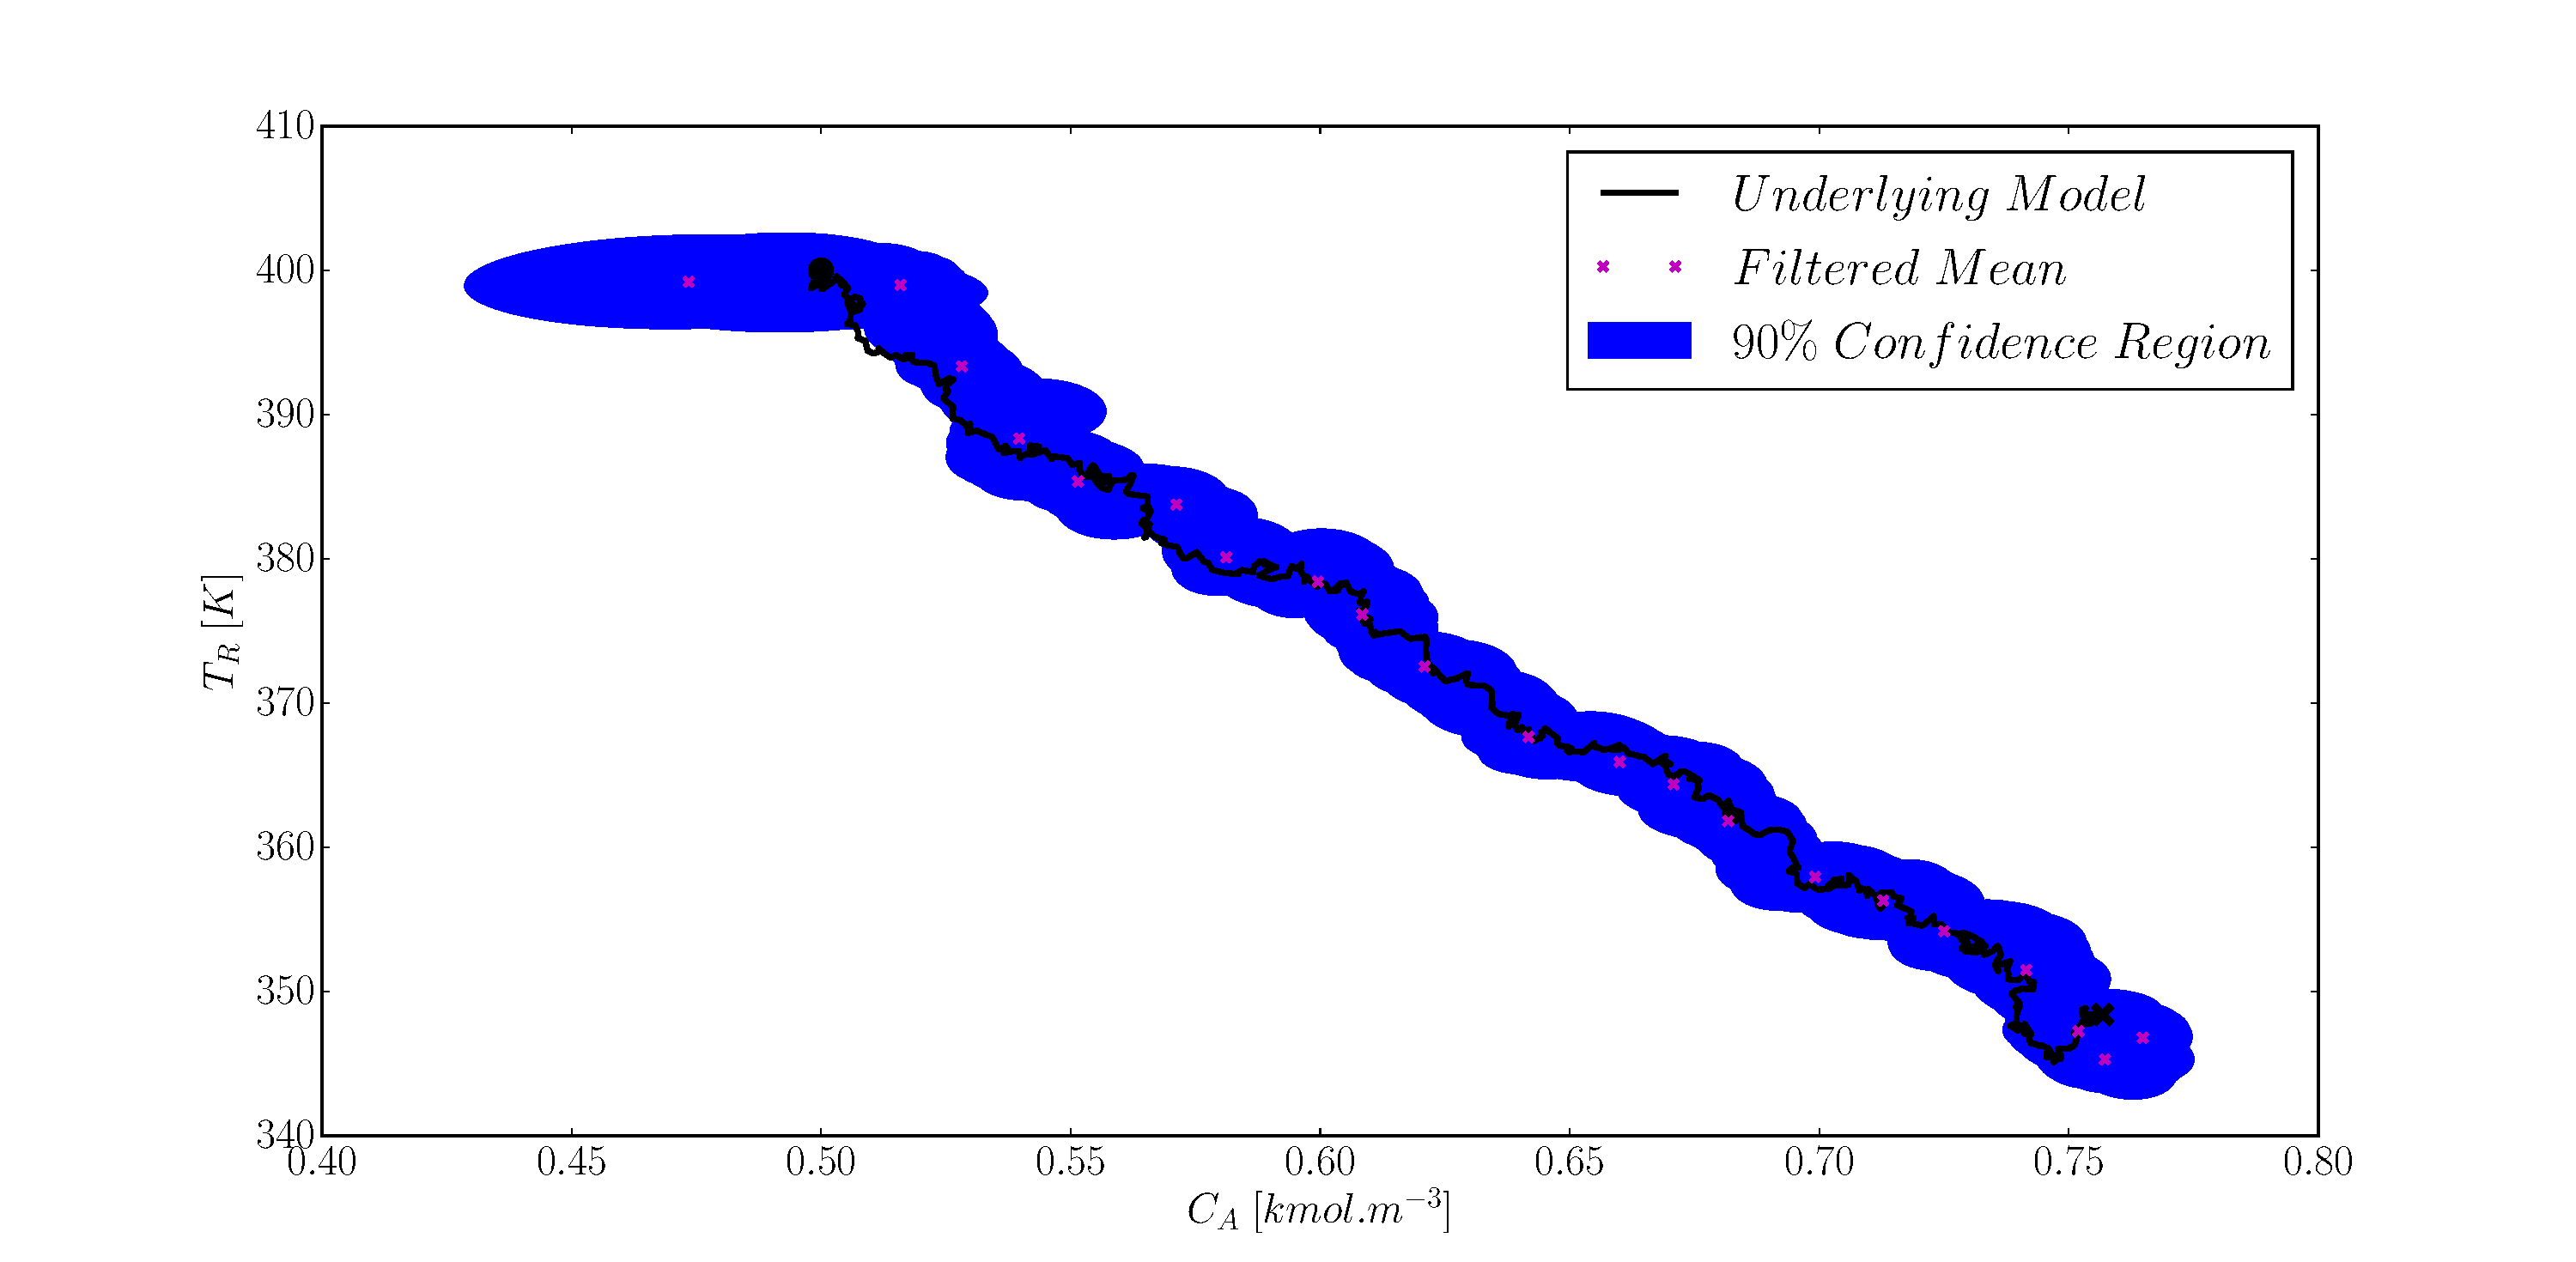
\includegraphics[width=\textwidth]{pf_m2_phase.pdf}
\caption{State space evolution of the particle filter on the nonlinear CSTR model with initial condition $(0.5, 450)$ and measuring both states. The filter uses 200 particles.}
\label{fig_pf_m2_phase}
\end{figure}
Finally we compare the particle filter to the Kalman filter using both temperature and concentration measurements. First we illustrate that if the underlying model is linear and the noise Gaussian the particle filter does no better than the Kalman filter. In figure \ref{fig_pf_kf_phase1} we see that both the particle filter and the Kalman filter are able to accurately estimate the posterior state distribution over time. Note that we have used 500 particles to meaningfully compare the distribution estimates (the more particles one uses in the particle filter the more accurate it becomes).
\begin{figure}[H] 
\centering
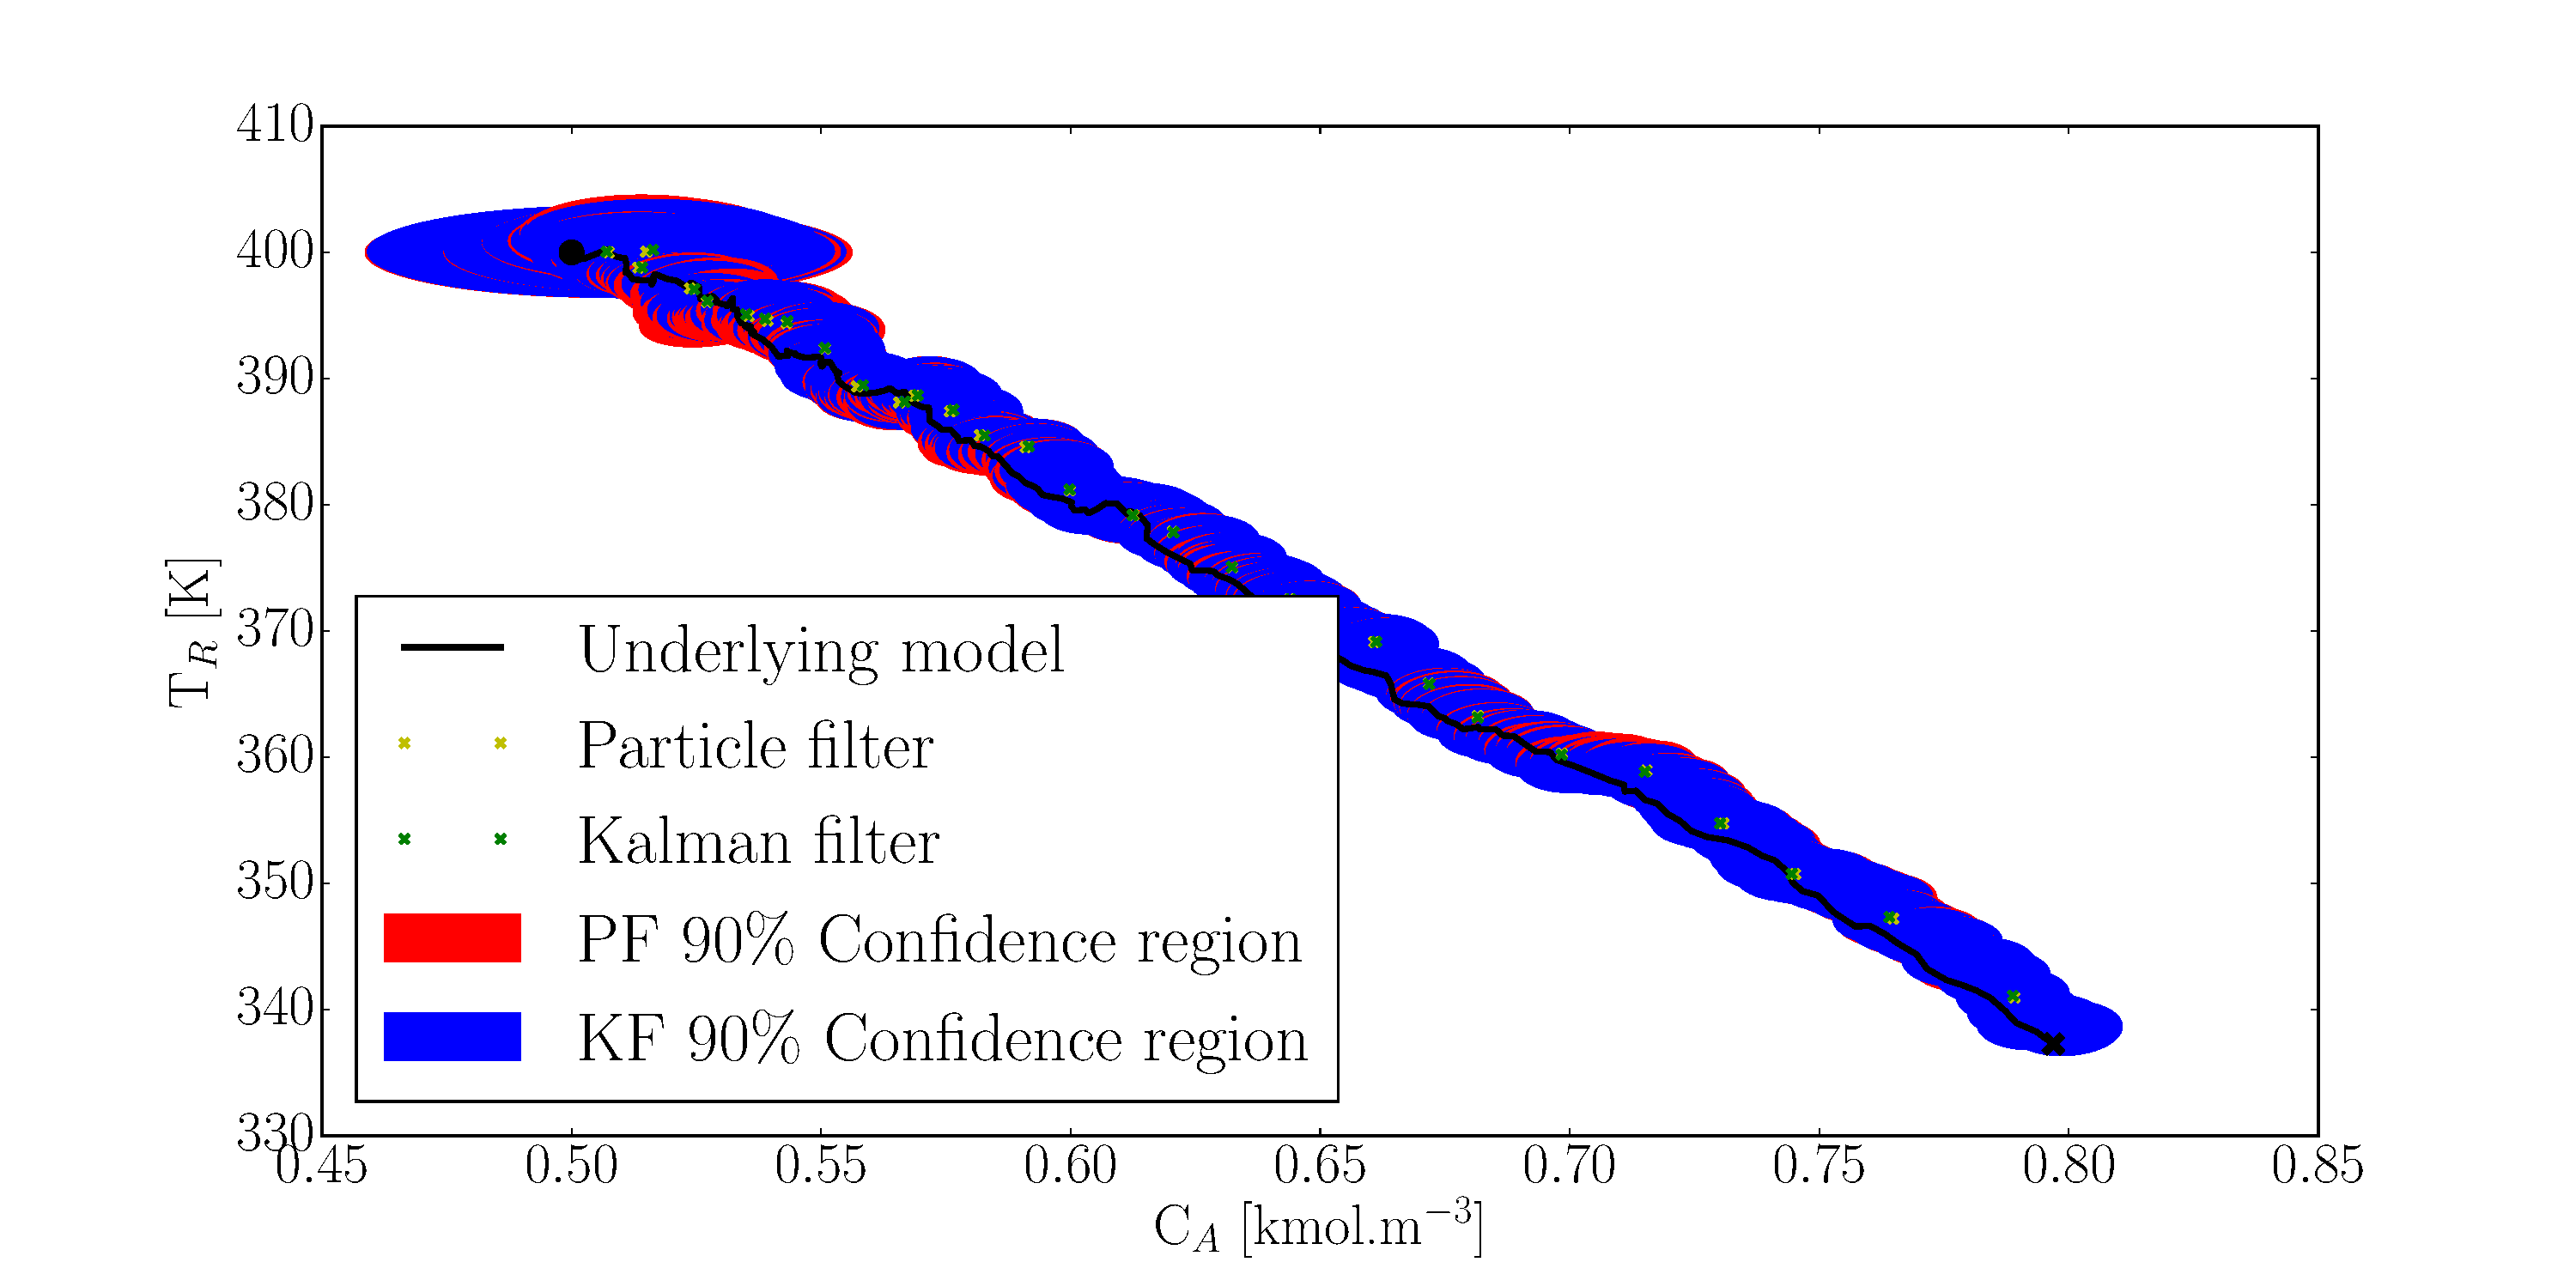
\includegraphics[width=\textwidth]{pf_kf_phase1.pdf}
\caption{State space evolution of the particle filter and the Kalman filter on the linear CSTR model with initial condition $(0.5, 400)$ and measuring both temperature and concentration. The particle filter uses 500 particles.}
\label{fig_pf_kf_phase1}
\end{figure}
The average concentration and temperature estimation errors for the particle filter is 0.93\% and 0.23\% respectively while the corresponding estimation errors for the Kalman filter is 0.97\% and 0.23\% respectively. Since the confidence region overlaps throughout the entire simulation it is clear that if the underlying model is linear there is no great difference between the two filters from an accuracy point of view. It does however makes sense, from a computational point of view, to use the Kalman filter: it is well known that the particle filter does not perform well in high dimensional problems\cite{snyder}. 

Next we consider the same comparison but change the underlying model to the full nonlinear CSTR as shown in figure \ref{fig_pf_kf_phase2}. The average concentration and temperature estimation errors for the particle filter is 0.83\% and 0.19\% respectively while the corresponding estimation errors for the Kalman filter is 4.50\% and 0.41\% respectively.
\begin{figure}[H] 
\centering
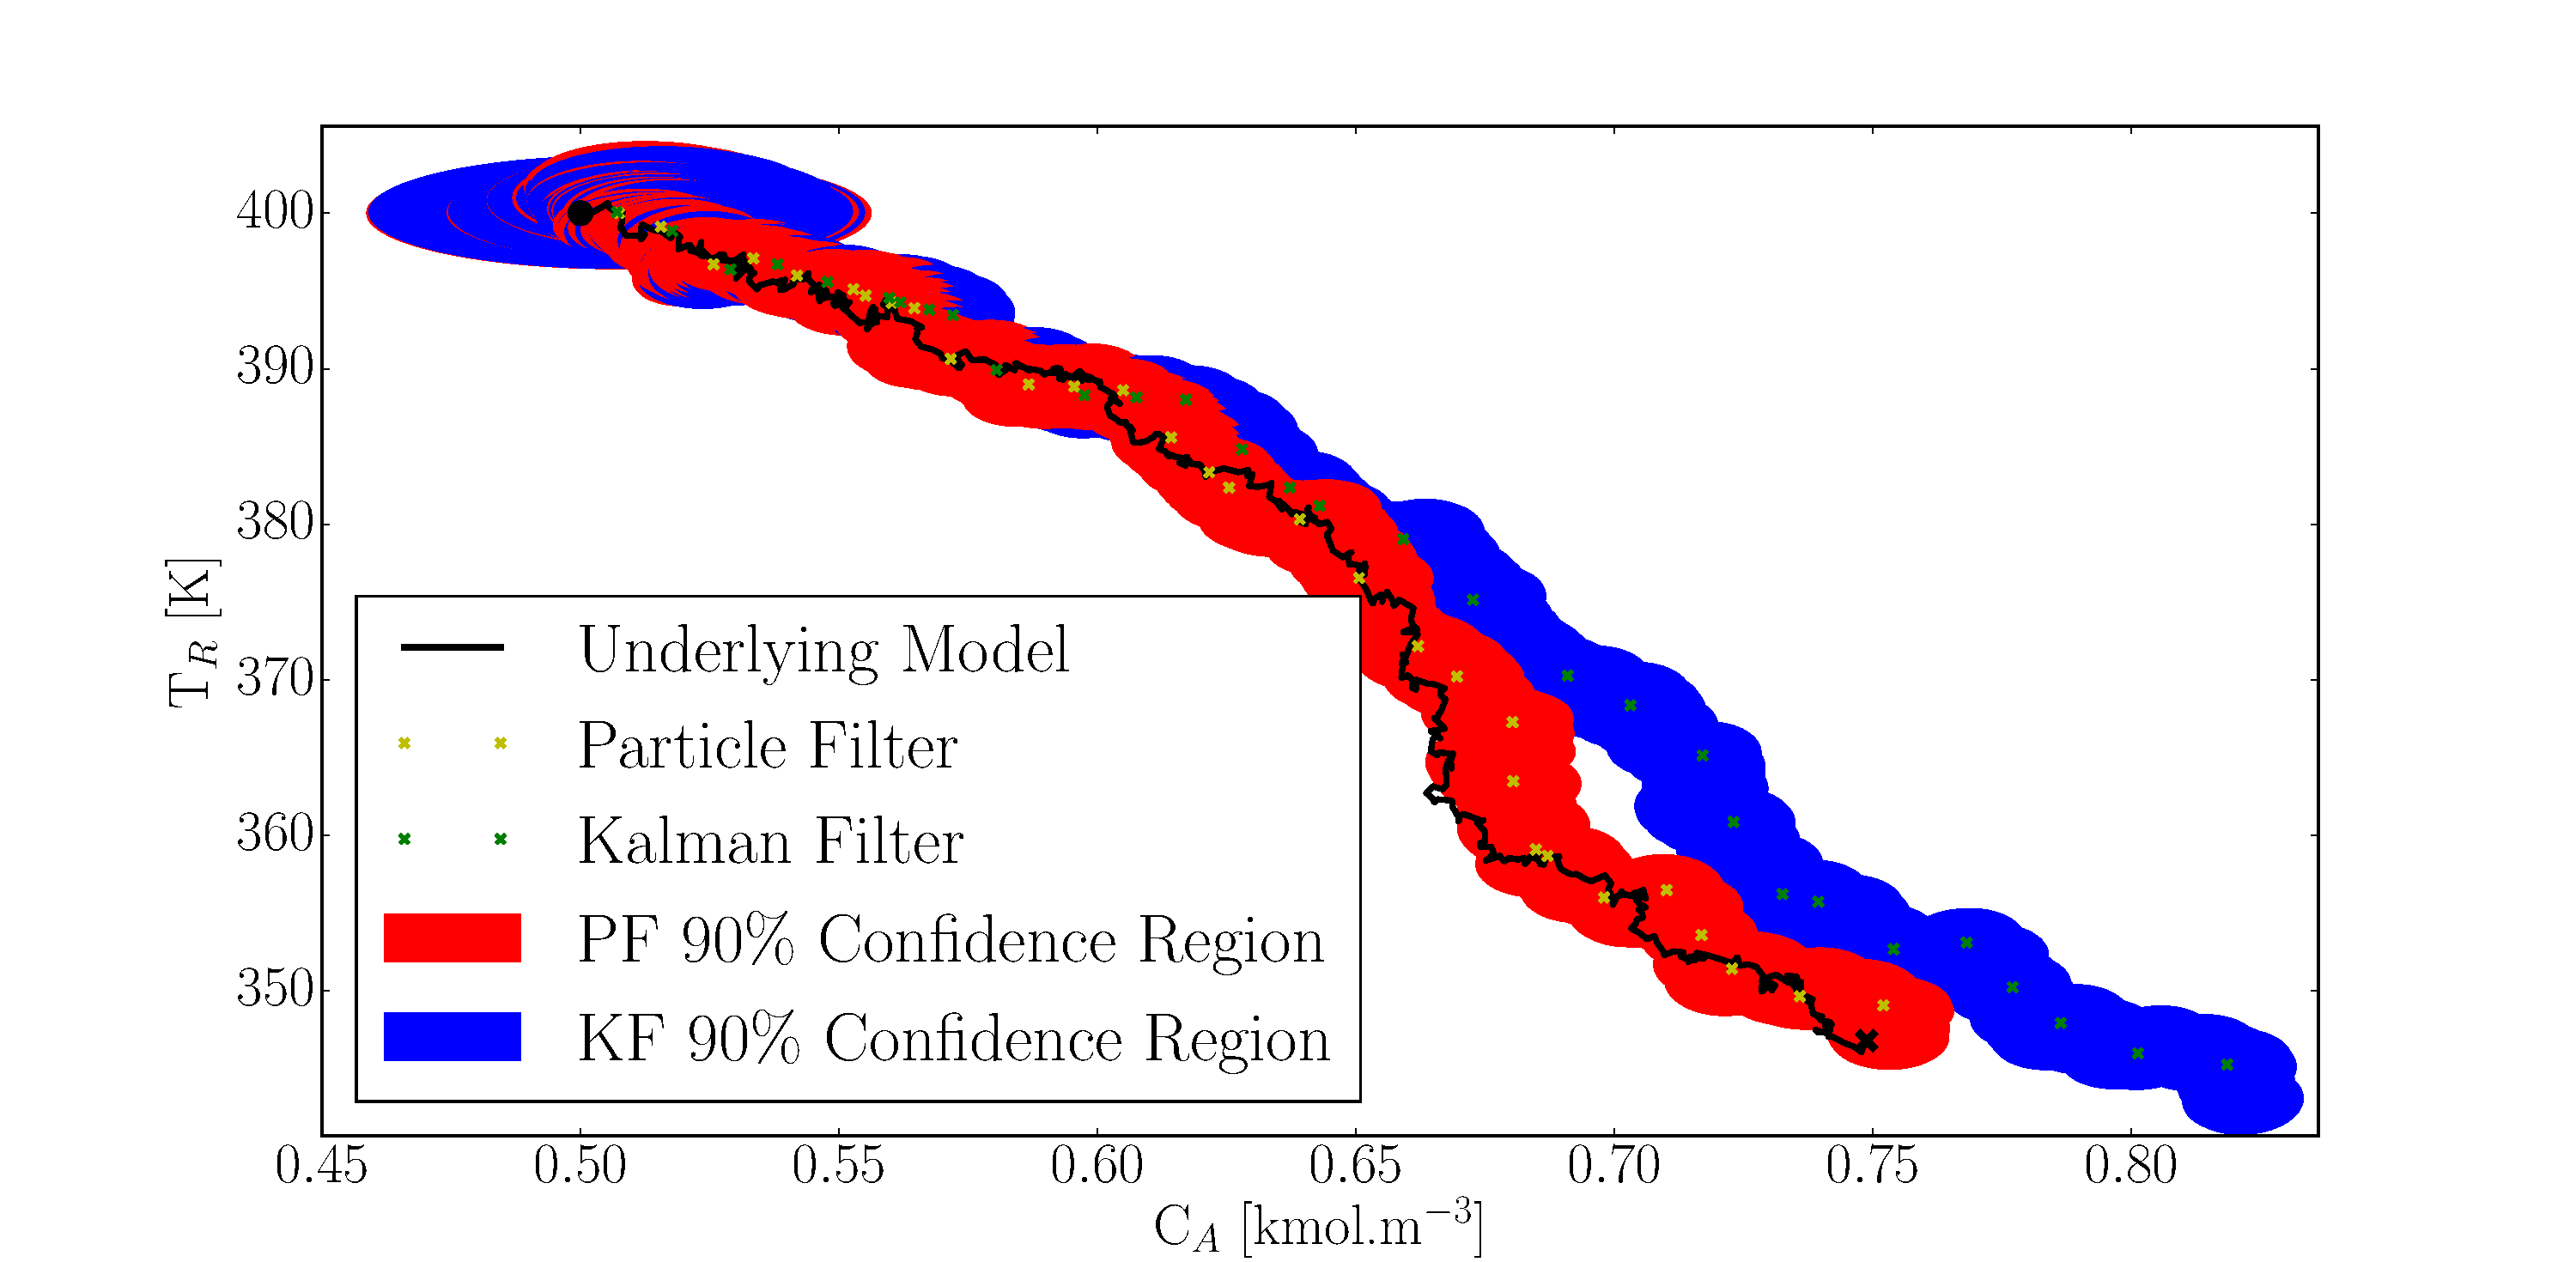
\includegraphics[width=\textwidth]{pf_kf_phase2.pdf}
\caption{State space evolution of the particle filter and the Kalman filter on the nonlinear CSTR model with initial condition $(0.5, 400)$ and measuring both temperature and concentration. The particle filter uses 500 particles.}
\label{fig_pf_kf_phase2}
\end{figure}
Inspecting figure \ref{fig_pf_kf_phase2} we see that throughout the simulation the particle filter's confidence region is smaller. Since we are using a significantly more accurate model for the particle filter this is not surprising. Additionally we see that the Kalman filter state estimates diverge from the true states as the model moves away from the region where the linear model is accurate. The same weakness in the Kalman filter was discussed in section \ref{sec_filtering_linmods} concerning the usage of the linear model.

Therefore, while the particle filter may be computationally more expensive to use it is a better filter if the system exhibits nonlinearity or non-normality. But, if the system is linear and normal one is better off using the standard Kalman filter.

In the next chapter we design model predictive controllers from within the framework of probabilistic graphical models.